%! Author = charon
%! Date = 2/8/24

\subsection{Die Fuzzingstatus Anzeige}\label{subsec:der-fuzzingstatus-bildschirm}
Der American Fuzzy Lop ist ausgestattet mit einer Statusanzeige, welcher den aktuellen Stand der Kampagne anzeigt.\\
\linebreak
\begin{figure}[h]
    \frame{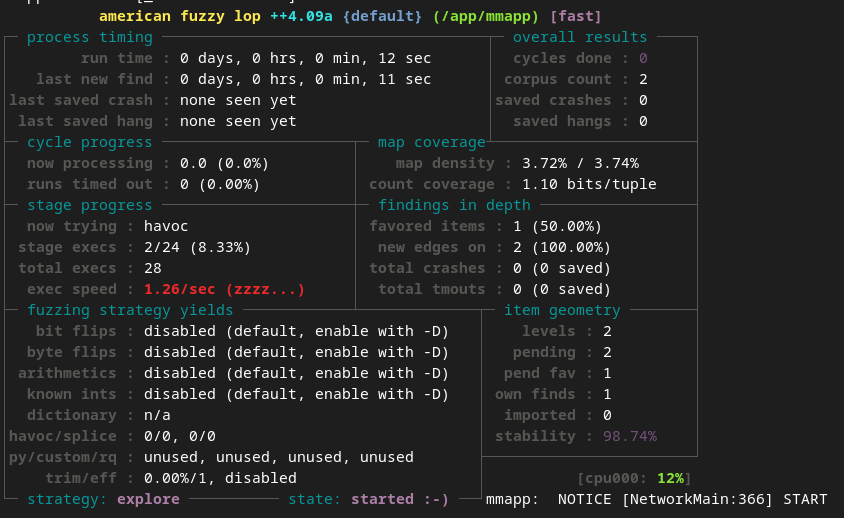
\includegraphics[width=\linewidth]{img/fuzzing-stauts}}
    \caption{Statusbildschirm von AFL}\label{fig:fuzzing-status}
\end{figure}\\
Der obere Teil der Statusbildanzeige wird als Statusleiste bezeichnet.
In ihr wird angezeigt, welche Version des~\gls{afl} verwendet wird, sowie in welchem Modus (hier \textit{\{default\}})
der Fuzzer gestartet wurde.
Als Nächstes steht die Applikation, welche derzeit gefuzzt wird.
Der Letzte, in der Statusleiste angezeigte, Wert beschreibt den Energiesparplan-Modus.
Im Normalfall wird der Modus \textit{fast} verwendet. \\
\linebreak
Desweiteren gibt es in der Statusanzeige ein Abteil mit dem Titel \textit{process timing}.
Ein besonderes Merkmal dieser Anzeige ist die Sektion \textit{last new find}.
Sie zeigt an, wann ein neuer Codepfad des Programms entdeckt wurde. \\
\linebreak
Die Sektion \textit{overall results} beinhaltet eine Übersicht verschiedener Ergebnisse der Kampagne.
Dazu gehört ein Zähler, welcher die Gesamtzahl der Iterationen aller Testcases beinhaltet.
Er wird erst hochgezählt, wenn alle im Korpus enthaltenen Testcases durchlaufen sind.
Darunter wird angegeben, wie viele Daten im Corpus vorhanden sind.
Anhand dessen kann man sehen, wie viel neuer Input von~\gls{afl} generiert wurde.
Zudem gibt es zwei weitere Zähler, die die Anzahl der Crashes und Hangs, die der Input verursacht hat, festhalten. \\
\linebreak
Der Abschnitt \textit{cycle progress} gibt Informationen über den derzeit verwendeten Input -- innerhalb eines Fuzzing-Zyklus --
mithilfe seiner~\gls{id}.
Außerdem wird hier auch die Anzahl an Eingaben festgehalten, welche die Kommunikation mit dem Programm zu einem Timeout führen.\\
\linebreak
Als Nächstes gibt es den Teil \textit{stage progress}.
Dieser gibt Auskunft über das aktuelle Verhalten des Fuzzers, sowie die derzeitige Phase, in dem sich der Fuzzer gerade befindet.
Das Feld \textit{now trying} steht dabei für die derzeit verwendete Mutationsstrategie des Inputs.
Das Schlüsselwort \textit{havoc} beschreibt, dass der Korpus derzeit mittels bitflips und Überschreiben von Integern innerhalb des
Testcases mutiert wird~\cite{stage-progress}.
Die weiteren Felder beschreiben die Ausführgeschwindigkeiten.
Sie zeigen ebenfalls auf, in welchem Zyklus sich der Fuzzer befindet und wie oft ein Durchlauf bereits ausgeführt wurde.\\
\linebreak
In der darauffolgenden Sektion \textit{findings in depth} werden Metriken für besondere Entdeckungen festgehalten.
Dazu gehören die Anzahl der Eingaben, die besonders gute Codepfadabdeckungen aufweisen (\textit{favored items}) oder besonders
weit in den Programmcode gelangen (\textit{new edges on}).
Außerdem werden die Anzahl der Inputs aufgezeichnet, die Crashes und Timeouts im Programm hervorrufen. \\
\linebreak
Die letzte -- für die Validierung der Kampagne wichtige -- Sektion \textit{path geometry} beinhaltet eine generalisierte Sicht
auf die Eingaben.
In diesem Abschnitt werden weitere Daten der Kampagne zur Analyse der Richtigkeit der Ausführung zusammengefasst.
Dazu gehört das Feld \textit{levels}, welches die Tiefe der Kampagne veranschaulicht.
In anderen Worten zeigt das Feld auf, wie viele Mutationszyklen die Eingaben bereits durchlaufen haben.
Die weiteren Felder \textit{pending} und \textit{pend fav} Zeigen auf welche Inputs von der Kampagne noch nicht zum Fuzzen
verwendet wurden, wobei \textit{fav} die von~\gls{afl} als favorisiert markierten Inputs sind.
Die favorisierten Inputs werden mit höherer Priorität von~\gls{afl} abgearbeitet.
Die nächsten beiden Felder \textit{own finds} und \textit{imported} zeigen die Anzahl der neu entdeckten Codepfade auf.
Hierbei anzumerken ist, dass unter Setups, mit zueinander parallel laufenden Fuzzern, \textit{own} die Codepfade der laufenden
Instanz sind und \textit{imported} die importierten Codepfade anderer Fuzzerinstanzen nach der Synchronisation derer miteinander aufzeigt.
Das letzte Datenfeld \textit{stability} misst die Zuverlässigkeit der Reaktion des Programms auf die vermittelten Eingaben.
Es zeigt die Anzahl der Testcases, welche bei mehrfachem Testen die gleichen Effekte/Codepfade erreicht haben.
Somit wird, wenn alle Testcases nach mehrfachem dasselbe Verhalten in einem Programm hervorgerufen haben, die Anzeige bei
\SI{100}{\percent} bleiben. \\
\linebreak
Die für den Tester interessanten Felder beschäftigen sich mit der Stabilität des Inputs, der Geschwindigkeit der Kampagne
und den Crashes.
Die Wahrscheinlichkeit, dass die Kampagne den gewünschten Effekt der Entdeckung eines Programmcrashs erzielt, hängt davon,
ab wie gut die Eingaben sind und wie schnell der Fuzzer das Programm ausführen kann.
Die Güte des Inputs wird daran bestimmt, ob ein Input eine möglichst hohe Programmpfadabdeckung hat und wie stabil das Programm
auf den Input reagiert.
Wenn ein Input beispielsweise bei jedem Durchlauf ein anderes Verhalten im Programm triggert, so ist dieser Input aufgrund
seiner unverifizierbarkeit wertlos.
Ein Input, der jedoch am Beispiel von mmapp einen Handler zur Verarbeitung dessen abläuft und möglichst weitere Programmfunktionen
auslöst, wird als guter Input bewertet.
Außerdem ist das Ziel eines Fuzzers Crashes zu finden, welche man potenziell ausnutzen kann.